\section{DREAM challenge networks with 100 nodes}
\label{app:dream_nets}

\begin{figure}[ht]
    \centering
    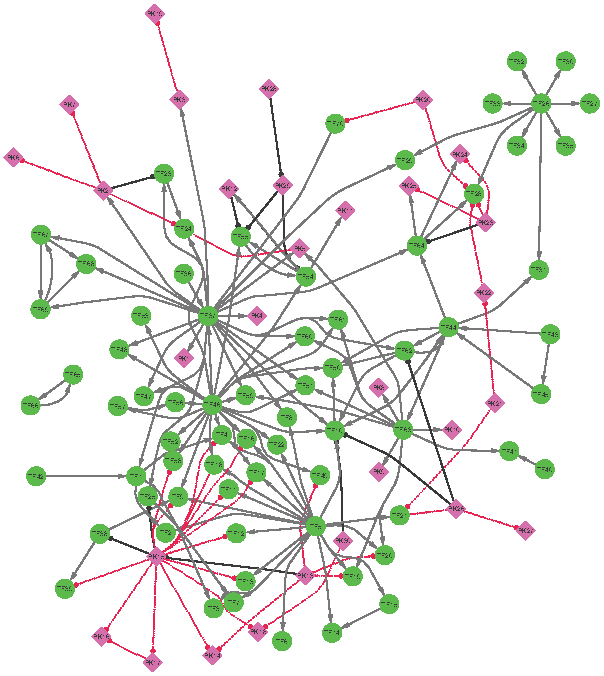
\includegraphics[width=\textwidth]{appendices/fig/net_100_1.pdf}
    \caption{\textbf{DREAM4 100 node network 1.} Edge color is grey for TF edges, black for detectable PK edges, red for undetectable PK edges.}
    \label{fig:dream4_net100.1}
\end{figure}

\begin{figure}[ht]
    \centering
    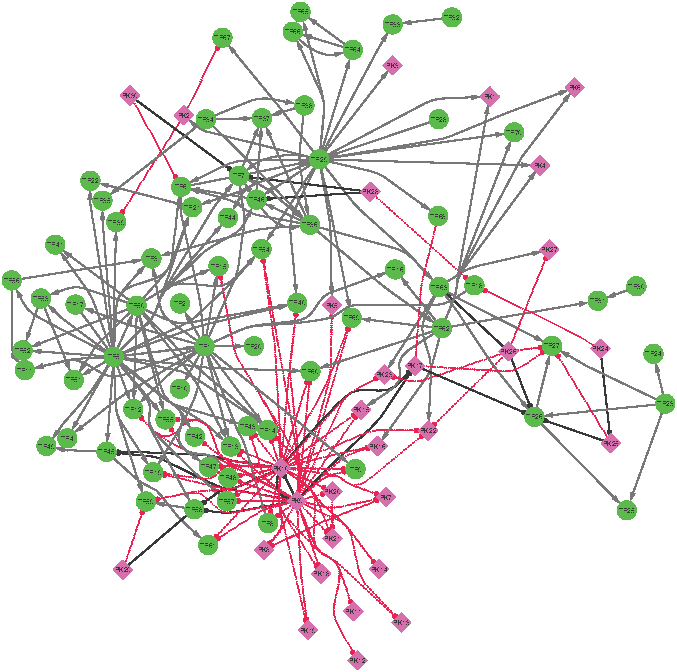
\includegraphics[width=\textwidth]{appendices/fig/net_100_2.pdf}
    \caption{\textbf{DREAM4 100 node network 2.} Edge color is grey for TF edges, black for detectable PK edges, red for undetectable PK edges.}
    \label{fig:dream4_net100.2}
\end{figure}

\begin{figure}[ht]
    \centering
    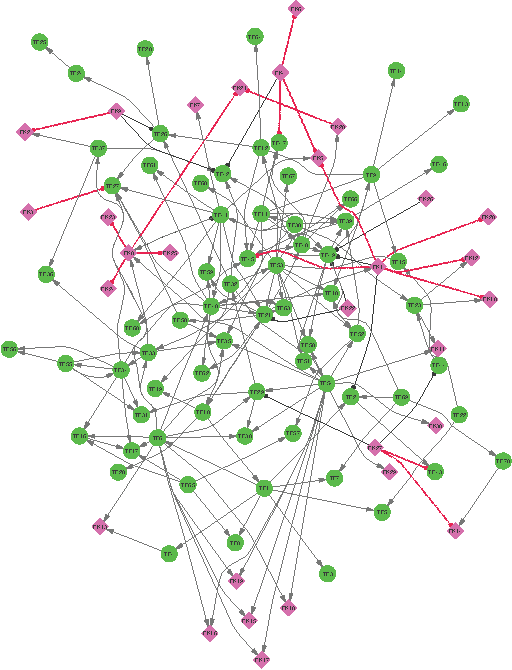
\includegraphics[width=\textwidth]{appendices/fig/net_100_3.pdf}
    \caption{\textbf{DREAM4 100 node network 3.} Edge color is grey for TF edges, black for detectable PK edges, red for undetectable PK edges.}
    \label{fig:dream4_net100.3}
\end{figure}

\begin{figure}[ht]
    \centering
    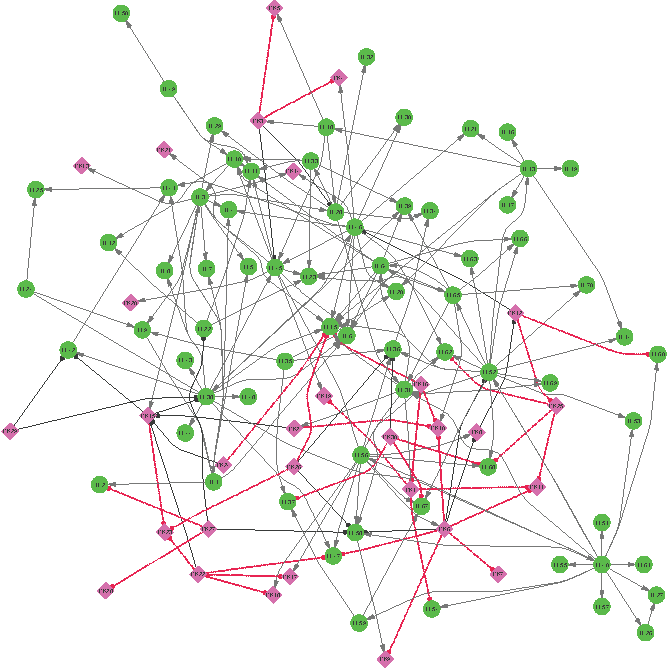
\includegraphics[width=\textwidth]{appendices/fig/net_100_4.pdf}
    \caption{\textbf{DREAM4 100 node network 4.} Edge color is grey for TF edges, black for detectable PK edges, red for undetectable PK edges.}
    \label{fig:dream4_net100.4}
\end{figure}

\begin{figure}[ht]
    \centering
    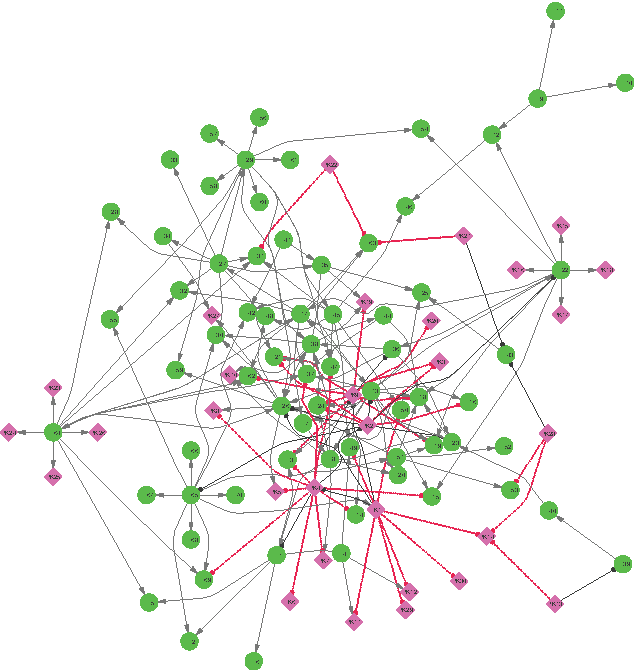
\includegraphics[width=\textwidth]{appendices/fig/net_100_5.pdf}
    \caption{\textbf{DREAM4 100 node network 5.} Edge color is grey for TF edges, black for detectable PK edges, red for undetectable PK edges.}
    \label{fig:dream4_net100.5}
\end{figure}